\chapter{Algorytmy oparte o A*}
\label{ch:astar}

Kiedy pojedynczy agent dokonuje znalezienia drogi do wyznaczonego celu, prosty algorytm A* sprawdza się bardzo dobrze. Jednak w przypadku, gdy wiele agentów porusza się w tym samym czasie, to podejście może się nie sprawdzić, powodując wzajemne blokowanie się i zakleszczenie jednostek. Rozwiązaniem tego problemu może być kooperacyjne znajdowanie tras. Roboty będą mogły skutecznie przemieszczać się przez mapę, omijając trasy wyznaczone przez inne jednostki oraz schodząc innym jednostkom z drogi, jeśli to konieczne. \cite{cooppath}

Zagadnienie znajdowania drogi jest ważnym elementem sztucznej inteligencji zaimplementowanej w wielu grach komputerowych. Chociaż klasyczny algorytm A* potrafi doprowadzić pojedynczego agenta do celu, to jednak dla wielu agentów wymagane jest zastosowanie innego podejścia w celu unikania kolizji. Algorytm A* może zostać zaadaptowany do replanowania trasy na żądanie, w przypadku wykrycia kolizji tras (Local Repair A* lub D*). Jednak takie podejście nie jest zadowalające pod wieloma względami. Na trudnych mapach z wieloma wąskimi korytarzami i wieloma agentami może to prowadzić do zakleszczenia agentów w wąskich gardłach lub do cyklicznego zapętlenia ruchu agentów. \cite{cooppath}

$TODO$ Które algorytmy tylko znajdują droge, a które rozwiązują problem kolizji

$TODO$ Większość z tych algorytmów wykorzystywana jest w grach. planowanie musi odbywać się szybko, szczególnie w grach (screen warcraft :))

\section{Algorytm A*}
A* jest algorytmem heurystycznym służącym do przeszukiwania grafu w celu znalezienia najkrótszej ścieżki. Algorytm ten jest powszechnie stosowany w zagadnieniach sztucznej inteligencji oraz w grach komputerowych \cite{mit_astar}. Jest modyfikacją algorytmu Dijkstry, wprowadza pojęcie funkcji heurystycznej $h(n)$. Wartość funkcji heurystycznej powinna określać przewidywaną drogę do węzła docelowego. W każdym kroku przeszukiwany jest węzeł o najmniejszej wartości funkcji $f(n)$.

\begin{gather}
 	f(n) = g(n) + h(n)
 	\label{eq_astar} 
\end{gather}
 gdzie:

 $g(n)$ - wartość kosztu, dokładna odgległość miedzy węzłem $n$ a węzłęm startowym

 $h(n)$ - heurystyka, przewidywana droga do węzła docelowego

 $n$ - węzeł, wierzchołek przeszukiwanego grafu

Dzięki takiemu podejściu najpierw sprawdzane są najbardziej "obiecujące" rozwiązania, co pozwala szybciej otrzymać rozwiązanie (w przeciwieństwie do algorytmu Dijkstry).
Algorytm kończy działanie w momencie, gdy napotka węzeł będący węzłem docelowym.
Dla każdego odwiedzonego węzła zapamiętywane są wartości $g(n)$, $h(n)$ oraz węzeł będący rodzicem w celu późniejszego odnalezienia drogi powrotnej do węzła startowego po napotkaniu węzła docelowego (por. rys. \ref{fig:image_astar2}).

\begin{figure}[H]
	\centering
	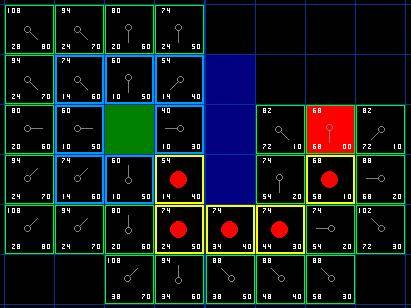
\includegraphics[width=10cm]{img/astar-t7}
	\caption{Przykład działania algorytmu A*. Źródło: \cite{astar2}}
	\label{fig:image_astar2}
\end{figure}

\subsection{Heurystyki}
Od wyboru sposobu obliczania heurystyki zależy czas wykonywania algorytmu oraz optymalność wyznaczonego rozwiązania.
Poniżej przedstawiono najczęściej wykorzystywane heurystyki.

$TODO$ Jeśli wartość heurystyki <= od rzeczywistej drogi, jaka musi zostać przebyta, to wyznaczona scieżka jest ścieżką optymalną (najkrótszą)
= admissible heuristic
An admissible heuristic never overestimates the distance to the goal. A* search with an
admissible heuristic is guaranteed to find the shortest path. However, there is a stronger
property, known as consistency [Russell03]. A consistent heuristic maintains the property
h(A) ≤ cost(A, B) + h(B) between all locations A and B. In other words, the estimated
distance doesn’t jump around between the locations along a path.
\cite{cooppath}

A* opiera się na heurystyce, która prowadzi przeszukiwaniem. Słaba heurystyka może prowadzić do zbędnego odwiedzania dodatkowych węzłów.

\subsubsection{Heurystyka Euklidesowa}
Dla dwuwymiarowej mapy heurystyka euklidesowa wyraża dokładną odległość między przeszukiwanym węzłem $(x_n, y_n)$ a węzłem docelowym $(x_g, y_g)$:
\begin{gather}
 	h(n) = \sqrt{(x_n - x_g)^2 + (y_n - y_g)^2}
 	\label{eq_astar_heu_euc} 
\end{gather}

\subsubsection{Heurystyka Manhattan}
W przypadku, gdy robot może poruszać się po mapie jedynie poziomo lub pionowo (nie na ukos) wystarczającym przybliżeniem jest metryka Manhattan:
\begin{gather}
 	h(n) = |x_n - x_g| + |y_n - y_g|
 	\label{eq_astar_heu_man} 
\end{gather}

$TODO$ Przykład z Pacmanem - screen - siatka podzielona na pola
zbliżenie do 0 sprowadza ją do ścieżki optymalnej (Dijkstry) - połowa heurystyki Manhattan daje możliwość wyznaczania trasy z uwzględnieniem zawijania mapy
The Manhattan distance is a consistent heuristic. The true distance heuristic is also consistent. (no chyba że zawijanie mapy)

\subsubsection{Heurystyka zerowa}
Przyjęcie heurystyki równej $h(n) = 0$ powoduje, że algorytm A* sprowadza się do algorytmu Dijkstry.

\section{Local Repair A*}
W algorytmie Local Repair A* (LRA*) każdy z agentów znajduje drogę do celu, używając algorytmu A*, ignorując pozostałe roboty oprócz ich obecnych sąsiadów. Roboty zaczynają podążać wyznaczonymi ścieżkami do momentu, aż kolizja z innym robotem jest nieuchronna. Wtedy następuje ponowne przeliczenie drogi pozostałej do przebycia, z uwzględnieniem nowo napotkanej przeszkody.

Możliwe (i całkiem powszechne \cite{cooppath}) jest uzyskanie cykli (tych samych sekwencji ruchów powtarzających się w nieskończoność), dlatego zazwyczaj wprowadzane są pewne modyfikacje, aby rozwiązać ten problem. Jedną z możliwości jest zwiększanie wpływu losowego szumu na wartość heurystyki. Kiedy agenci zachowują się bardziej losowo, prawdopodobne jest, że wydostaną się z problematycznego położenia i spróbują podążać innymi ścieżkami.

Algorytm ten ma jednak sporo poważnych wad, które szczególnie ujawniają się w trudnych środowiskach z dużą liczbą przeszkód. Wydostanie się z zatłoczonego wąskiego gardła może trwać bardzo długo. Prowadzi to również do ponownego przeliczania trasy w prawie każdym kroku. Wciąż możliwe jest również odwiedzanie tych samych lokalizacji w wyniku zapętleń.

$TODO$ Jest to przykład rozproszonej struktury organizacyjnej - Podejmowanie decyzji przez roboty lokalnie (+ centralnie)???

\section{Algorytm D*}
D* ({\it Dynamic A* Search}) jest przyrostowym algorytmem przeszukiwania. Jest modyfikacją algorytmu A* pozwalającą na szybsze replanowanie trasy w wyniku zmiany otoczenia (np. zajmowania wolnego pola przez innego robota). Wykorzystywany jest m.in. w nawigacji robota do określonego celu w nieznanym terenie. Początkowo robot planuje drogę na podstawie pewnych założeń (np. nieznany teren nie zawiera przeszkód). Podążając wyznaczoną ścieżką, robot odkrywa rzeczywisty stan mapy i jeśli to konieczne, wykonuje ponowne planowanie trasy na podstawie nowych informacji.
Często wykorzystywaną implementacją (z uwagi na zoptymalizowaną złożoność obliczeniową) jest wariant algorytmu {\it D* Lite} \cite{dstarlite}.

\section{Cooperative A*}
$TODO$
Cooperative A* jest algorytmem do rozwiązywania problemu kooperacyjnego znajdowania tras.
Metoda może być również nazywana czasoprzestrzennym algorytmem A* ({\it time-space A* search})
Zadanie planowania jest rozdzielone na serię pojedynczych poszukiwań dla poszczególnych agentów.
Pojedyncze poszukiwania są wykonywane w trójwymiarowej czasoprzestrzeni i biorą pod uwagę zaplanowane ścieżki przez pozostałych agentów.
Akcja wykonania postoju (pozostania w tym samym miejscu) jest uwzględniona w zbiorze akcji możliwych do wykonania.
Po przeliczeniu dróg dla każdego agenta, stany zajętości pól są zaznaczane w tablicy rezerwazji (ang. Reservation table).
Pozycje w tej tablicy są uważane jako pola nieprzejezdne i w efekcie są omijane podczas przeszukiwania przez późniejszych agentów. \cite{cooppath}

Należy zaznaczyć, że planowanie dla każdego agenta odbywa się sekwencyjnie według przydzielonych priorytetów.
Algorytm ten jest podatny na zmianę kolejności agentów. Odpowiedni dobór priorytetów może wpłynąć na wydajność algorytmu oraz jakość uzyskanego wyniku.

\subsection{Trzeci wymiar}
$TODO$
Do rozwiązania problemu kooperacyjnego znajdowania dróg algorytm przeszukiwania potrzebuje mieć pełną wiedzę na temat przeszkód oraz jednostek na mapie.
Aby zapisać tą informację potrzeba rozszerzyć mapę o trzeci wymiar - czas. 
Pierwotną mapę będziemy nazywac mapą przestrzenną, natomiast nową - czasoprzestrzenną mapą. \cite{cooppath}

Zagadnienie sprowadza się do przeszukiwania grafu, w którym każdy węzeł ma przypisane 3 wielkości: położenie x, położenie y oraz czas.
Podczas gdy zakres wielkości x i y jest znany i wynika z rozmiarów mapy oraz podziału jej wymiarów na dyskretne pola, to jednak określenie wymiaru czasu może być trudnym zagadnieniem.
Wymiar czasu możemy również zdyskretyzować i przyjać, że najmniejsza jednostka jest czasem, jaki zajmuje robotowi przejście z jednego pola na sąsiednie (poziomo lub pionowo). Natomiast górną granicą czasu powinna być maksymalna liczba ruchów potrzebna do dotarcia do celu przez ostatniego robota. Wybór za małej liczby może spowodować, że algorytm nie znajdzie drogi dla niektórych agentów, z kolei za duża granica czasu mocno wydłuża czas obliczeń. Rozwiązanie tego problemu zostało opisane w późniejszym podrozdziale \ref{ch:hier_cooperative_a}.

Wprowadzenie trzeciego wymiaru powoduje również konieczność zmian w doborze odpowiedniej heurystyki odpowiedzialnej za oszacowanie drogi pozostałej do celu.

\subsection{Tablica rezerwacji}
Tablica rezerwacji (ang. {\it Reservation Table}) reprezentuje wspódzieloną wiedzę o zaplanowanych ścieżkach przez wszystkich agentów.
Jest to informacja o zajętości każdej z komórki na mapie w danym miejscu i określonym czasie. \cite{cooppath}

Jak tylko agent zaplanuje trasę, każda komórka odpowiadająca ścieżce zaznaczana jest jako zajęta w tablicy rezerwacji.

W prostej implementacji tablica rezerwacji jest trójwymiarową kostką (dwa wymiary przestrzenne i jeden wymiar czasu).
Każda komórka kostki, która jest przecinana przez zaplanowaną przez agenta ścieżkę, jest zaznaczana jako nieprzejezdna przez określony czas trwania. W ten sposób zapobiega to planowania kolizyjnych tras przez pozostałych agentów.

\begin{figure}[H]
	\centering
	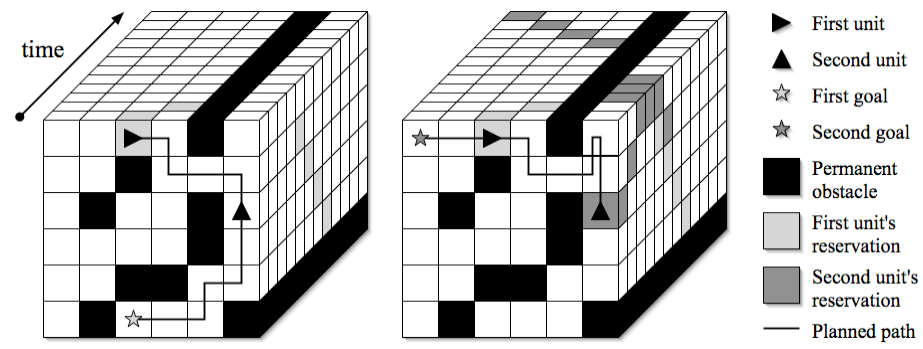
\includegraphics[width=10cm]{img/reservation-table}
	\caption{Dwie jednostki kooperacyjnie poszukujące tras. (A) Pierwsza jednostka znajduje ścieżkę i zaznacza ją w tablicy rezerwacji. (B) Druga jednostka znajduje ścieżkę, uwzględniając istniejące rezerwacje pól, również zaznaczając ją w tablicy rezerwacji. Źródło: \cite{cooppath}}
	\label{fig:img_reservation-table}
\end{figure}

W ogólności poszczególni agenci mogą mieć różną prędkość lub rozmiary, zatem tablica rezerwacji musi mieć możliwość zaznaczenia dowolnego zajętego obszaru. Zostało to przedstawione na rysunku \ref{fig:img_reservation-table-2}.

\begin{figure}[H]
	\centering
	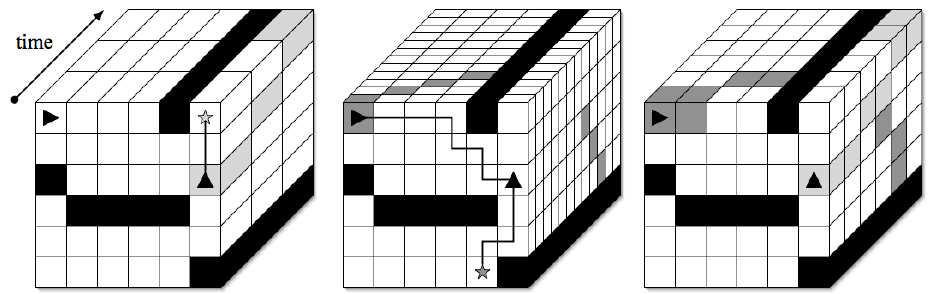
\includegraphics[width=10cm]{img/reservation-table-2}
	\caption{Czasoprzestrzenna mapa może różnić się od tablicy rezerwacji. (A) Powolna jednostka ma "głębokie" komórki na czasoprzestrzennej mapie. (B) Szybka jednostka ma "płytkie" komórki. (C) Tablica rezerwacji jest współdzielona między wszystkimi agentami, dlatego powinna być odpowiednio dopasowana do wszystkich agentów. Źródło: \cite{cooppath}}
	\label{fig:img_reservation-table-2}
\end{figure}

Jeśli tylko mała część z całej tablicy rezerwacji będzie markowana jako zajęta, wydajniej jest zaimplementować ją jako tablicę typu {\it hash table}. Daje to zaletę oszczędności pamięci poprzez pamiętanie jedynie współrzędnych $(x, y, t)$ zajętych pól.

Niestety taki sposób wykorzystania tablicy rezerwacji w pewnych sytuacjach nie zapobiega zderzeniom czołowym jednostek zmierzających w przeciwnych kierunkach.
Jeśli jedna jednostka zarezerwowała komórki $(x, y, t)$ i $(x + 1, y, t + 1)$, nic nie stoi na przeszkodzie, aby kolejna jednostka mogła zarezerwować komórki $(x + 1, y, t)$ i $(x, y, t + 1)$. Ten problem może być rozwiązany poprzez zajmowanie (rezerwowanie) dwóch sąsiednich komórek w tym samym czasie $t$ podczas ruchu robota.

\section{Hierarchical Cooperative A*}
\label{ch:hier_cooperative_a}
$TODO$
The second generic method for improving a heuristic based on abstractions of the state space is to use Hierarchical A*.
With this approach the abstract distances are computed on demand. The hierarchy in this case refers to a
series of abstractions of the state space, each more general
than the previous, and is not restricted to spatial hierarchy.
The choice of hierarchy is critical, and that
large hierarchies may in fact perform worse than small, sim-
ple hierarchies.

Hierarchical Cooperative A* (HCA*) uses a simple hier-
archy containing a single domain abstraction, which ignores
both the time dimension and the reservation table. In other
words, the abstraction is a simple 2-dimensional map with
all agents removed. Abstract distances can thus be viewed
as perfect estimates of the distance to the destination, ig-
noring any potential interactions with other agents. This is
clearly an admissible and consistent heuristic. Furthermore,
the inaccuracy of the heuristic is determined only by the dif-
ficulty of interacting with other agents (how much the agent
must deviate from the direct path to avoid other agents).

A fourth approach is introduced here, which is to use a Reverse
Resumable A* (RRA*) search in the abstract domain.
The RRA* algorithm executes a modified A* search in a
reverse direction. The search starts at the agent’s goal G,
and heads towards the agent’s initial position O. Instead
of terminating at O, the search continues until a specified
node N is expanded.

HCA* is just like CA* with a more sophisticated heuris-
tic, using RRA* to calculate the abstract distance on demand.
\cite{cooppath}

\section{Windowed Hierarchical Cooperative A*}
$TODO$
One issue with the previous algorithms is how they termi-
nate once the agents reach their destination. If an agent sits
on its destination, for example in a narrow corridor, then
it may block off parts of the map to other agents. Ideally,
agents should continue to cooperate after reaching their des-
tinations, so that an agent can move off its destination and
allow others to pass.

A second issue is the sensitivity to agent ordering. Al-
though it is sometimes possible to prioritise agents globally
(Latombe 1991), a more robust solution is to dynamically
vary the agent order, so that every agent will have the high-
est priority for a short period of time. Solutions can then
be found which would be unsolvable with an arbitrary, fixed
agent order.

A simple solution to all of these issues is to window the
search. The cooperative search is limited to a fixed depth
specified by the current window. Each agent searches for a
partial route to its destination, and then begins following the
route. At regular intervals (e.g. when an agent is half-way
through its partial route) the window is shifted forwards and
a new partial route is computed.

To ensure that the agent heads in the correct direction,
only the cooperative search depth is limited to a fixed depth,
whilst the abstract search is executed to full depth. A win-
dow of size w can be viewed as an intermediate abstraction
that is equivalent to the base level state space for w steps,
and then equivalent to the abstract level state space for the
remainder of the search. In other words, other agents are
only considered for w steps (via the reservation table) and
are ignored for the remainder of the search.
\cite{cooppath}


$TODO$
One example of a decoupled approach is HCA* [Silver,
2005]. HCA* employs a reservation table for timestep-
location pairs. The algorithm chooses a fixed ordering of
agents, and plans a path for each agent in turn that avoids con-
flicts with previously computed paths by checking against the
reservation table. Unfortunately, in over half of our bench-
mark instances, some agents never reach their destinations
because the paths found for previous agents in the fixed or-
der can make finding paths for subsequent agents impossi-
ble. Using a windowed search, Silver’s WHCA* mitigates
this problem at the cost of solution quality and running time.
\cite{completealgo_standley}

$TODO$
WHCA* (Windowed Hierarchical Cooperative A*) uses a temporal-spatial search, that
is, a node in the search tree is not only defined by the position, but is also defined by the
time the agent will be there. The search is also windowed; this means that it is performed
a fixed number of steps into the future, and the most promising node at the edge of this
window is selected.
To plan all the agents' paths at the same time carries an all-to-high computational cost[9].
Instead, a reservation table is used. The path of every agent is planned independently, and
every position and time that a node is blocked is recorded in the reservation table. This is
a reasonable approach to decrease the computational costs involved, which although it may
not solve all problems, will be able to solve many of them.
To focus the search, a spatial reverse A* search is used as heuristic for the temporal-
spatial search. That is, it is used to calculate the exact distance from a node to the goal,
excluding the influence other agents may have on this distance. This generally focuses the
search a lot, as this is often a very high-quality heuristic. It gets worse with a higher level
of congestion in the environment.
However, this reverse A* search leads to a high initial cost when performing the first
windowed temporal-spatial search, as it needs to perform a full A* search from the goal
to the start (as well as to some nodes neighbouring the start), but the cost for subsequent
searches will be lower.
\cite{rtcooppathfinding}

Windowed Hierarchical Cooperative A*:
• Cooperative A*
• Hierarchical Heuristic
• Windowed cooperation

Use a hash table to store time-space indexed reservations
• Reserve / Free a space/time cell

$TODO$ Clearance-based Pathfinding and Hierarchical Annotated A* Search - używane, gdy jednostki zajmują różne obszary, ale chyba tylko dla jednej jednostki (nie cooperative)